\chapter{绪论}
\label{chap:introduction}

\fontsize{12bp}{14.4pt}


\section{光学微腔简介}
光学谐振腔将光局域在一定的空间内。高品质因子谐振腔将光子长时间局域在一定空间内,使得光在其中循环,光场强度随之叠加。相干叠加的性质导致谐振腔仅允许特定频率的光存在,称之为模式。谐振模式光场受到极大地增强,加强了光与物质相互作用,催生了一系列研究领域$~^{[6]}$:腔QED,腔光力学,微腔传感,微腔光频梳$~^{[5]}$。模式体积$V$描述了微腔的空间局域能力,品质因子$Q$描述了时间局域能力,是微腔最重要的两个指标$~^{[14]}$。$Q$越大,$V$越小,则光与物质相互作用越强。
\section{光学频率梳简介}
光学频率梳在频域上是等间距的谱线,因此得名“梳”。时域上,它是等间隔的脉冲。
\begin{figure}[htbp]
    \centering
    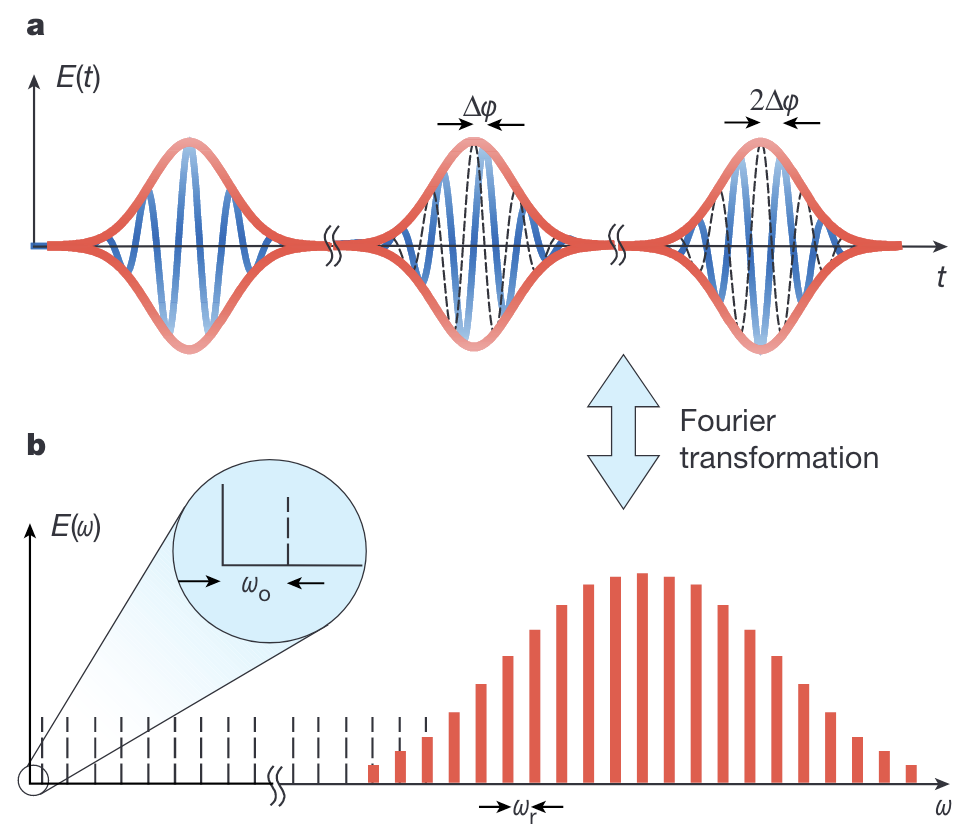
\includegraphics[width=0.7\linewidth]{figure/fig_3.png}
    \caption{光学频率梳。a.时域上为等间隔的脉冲包络,实际电场有着相位偏差。b.频域上为等间距的梳齿,在延拓到零频处有偏移。}
    \label{fig:enter-label}
\end{figure}
由于脉冲的群速度和相速度差别,光频段等间隔的谱线延伸到零频附近时会有偏移$f_{CEO}$。重复频率$f_{rep}$容易获得;通过自参考,也可测得偏移频率$f_{CEO}$。\\
由此,各模式的频率即可写为:
\[f_n = f_{CEO} + n * f_{rep}\]
$n$的量级为$10^6$。光学频率梳相干地连接了电子学和光学两个领域,催生了一系列研究:光钟,光谱探测,低噪声微波。\\
\begin{figure}[htbp]
    \centering
    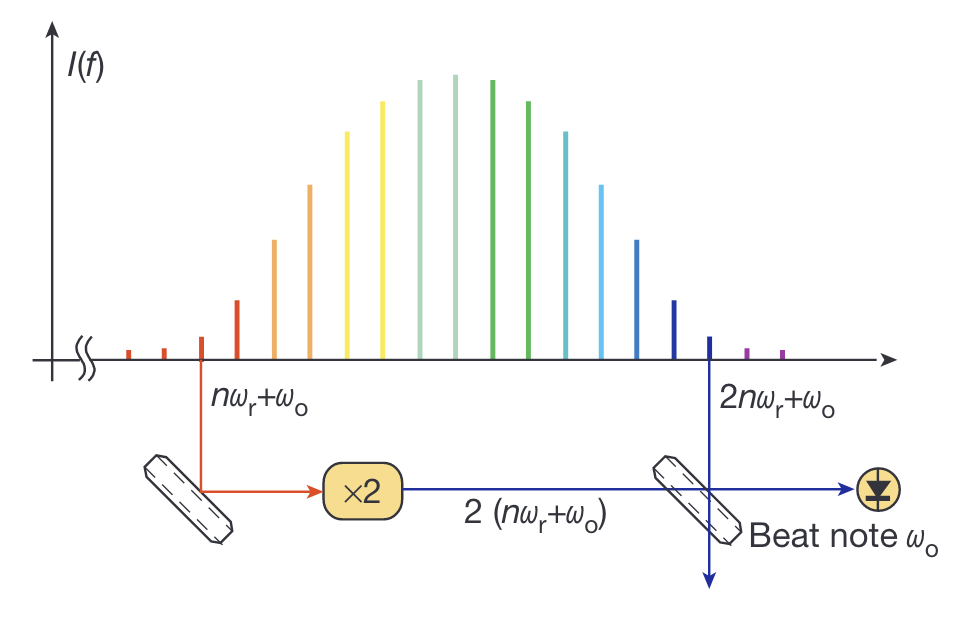
\includegraphics[width=0.7\linewidth]{figure/fig_2.png}
    \caption{自参考技术。选出跨倍频程光梳$~^{[4]}$的$n$和$2n$模式,将低频模式倍频,即可与高频模式拍出光梳的偏移频率。}
    \label{fig:enter-label}
\end{figure}
\subsection{Kerr梳}
Kerr梳利用材料的三阶非线性效应,通过简并和非简并四波混频在泵浦光两边级联产生等间距的梳尺$~^{[8]}$。对于三阶非线性,$Q^2/V$表征了非线性的强度。亮孤子态是一种锁模态,时域上是稳定的脉冲。孤子通过平衡损耗与非线性增益,色散与Kerr效应而保持稳定,存在于反常群速度色散的腔中。$~^{[10]}$\\
\begin{figure}[htbp]
    \centering
    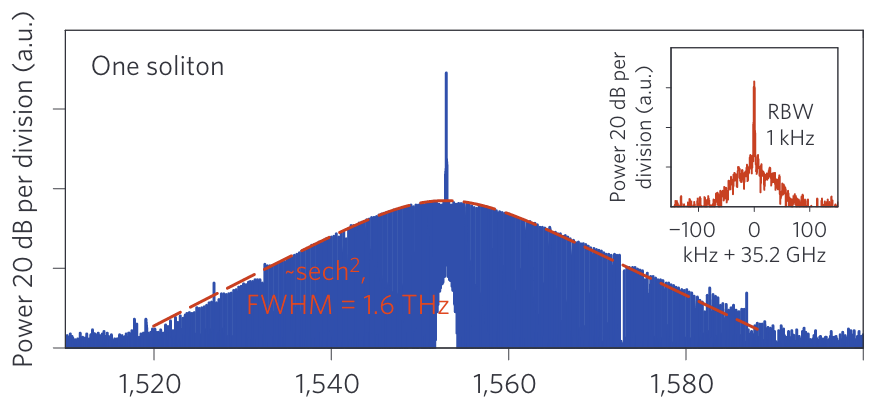
\includegraphics[width=0.7\linewidth]{figure/fig_6.png}
    \caption{单孤子态。}
    \label{fig:enter-label}
\end{figure}
进入孤子态通常需要复杂的泵浦频率或强度调节过程。
\subsection{电光梳}
电光梳通过光学回路中的相位调制器产生。泵浦光受到调制而产生边带,当调制频率与重频相等时,边带也被谐振加强且受到调制,又产生新边带,如此级联形成了电光梳。\\
\begin{figure}[htbp]
    \centering
    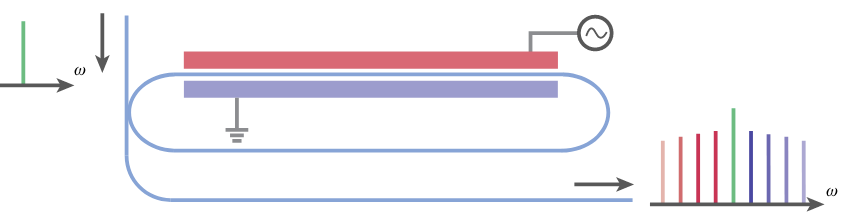
\includegraphics[width=0.7\linewidth]{figure/fig_5.png}
    \caption{电光梳。腔内谐振的电光调制将部分输入单频光转化为输出的级联边带。}
    \label{fig:enter-label}
\end{figure}
电光梳结构简单,但早期电光梳的转换效率和展宽受制于弱电光作用强度和无法控制色散。
\subsection{集成锁模激光器——研究动机}
锁模激光器是最早用来产生超短脉冲的结构。锁模激光器在稳态下,回路中也存在着孤子,并同时满足增益-损耗,色散-非线性的平衡。增益来源于受到泵浦的增益介质,非线性则是锁模的关键。早期,锁模激光器采用强度调制等主动锁模方式;如今大部分则依靠饱和吸收体等被动锁模方式运行。\\
由于集成平台上缺少成熟的引入增益介质的工艺,因此集成锁模激光器领域尚处在研究的早期阶段。
\section{铌酸锂简介}
集成光子学平台有很多:硅,氮化硅,氮化铝等等,但只有铌酸锂同时具有1.低损耗,2.高非线性,3.快速响应的电光调制。$~^{[17]}$因此铌酸锂是进行光电研究的极佳材料。铌酸锂在光纤光学中很常见:电光调制器、频率转换器等等。但由于铌酸锂难以进行微纳加工,传统的铌酸锂波导对与光场的局域性差。直到最近十年,铌酸锂平面波导工艺的突破,让铌酸锂再次成为集成光子学研究的活跃平台。
\subsection{二阶非线性效应}
铌酸锂的晶体结构为3m点群,无中心反演对称性,因此具有二阶非线性效应。\\
二阶非线性效应也叫做线性电光效应,通过Pockels矩阵描述,可以简写为:
\[\Delta \epsilon_{ij} = -\Sigma_k epsilon_{ii}\epsilon_{jj}r_{ijk}E_k/\epsilon_0\]
铌酸锂中最大的线性电光系数为$r_{333} = 31pm/V$,使用这一系数需要使得外加微波电场和光场的方向都与晶体z轴平行。
\subsection{三阶非线性效应}
铌酸锂的非线性折射率为$n_2 = 1.8*10^{-19}m^2/W$,与氮化硅$2.5*10^{-19}$为一个量级。因此也可以在铌酸锂上产生Kerr梳。
\subsection{光折变}
光折变时受激发载流子的空间不均匀分布形成的电场而在二阶非线性材料中产生的局部折射率变化。由于波导内外光强差异大,因此薄膜铌酸锂波导有着很强的光折变效应。\\
光折变产生的折射率变化方向$~^{[9]}$与热效应$~^{[3]}$相反,弛豫时间更长。两者的相互作用可使Kerr孤子自启动。
% \section{本文内容安排}
% 本文共六章节,
